\documentclass[11pt,a4paper,english,oneside]{book}

%----------------------------------------------------------------------------------------
% THESIS SETTINGS - ADAPT
%----------------------------------------------------------------------------------------
% Depending on your program, (un)comment the following lines

% Are you in the Quant finance program?
\newif\ifQF % default behaviour is false, so NOT in QF - always leave uncommented!
% \QFtrue % Uncomment if you are in the QF program, if not leave it out

% Pick One option
\newcommand{\thesis}{Momentum Anaylsis}
% \newcommand{\thesis}{Master}


% ==========================================================================================
% PREAMBLE
% ==========================================================================================
%----------------------------------------------------------------------------------------
% GENERAL  - PACKAGES
%----------------------------------------------------------------------------------------
% GENERAL
\usepackage{etex} %Because of many packages --> Extended TeX.
\usepackage[utf8]{inputenc} %Due to vowels.
% \usepackage[british]{babel} %Define the language style.

%Load some mathematical packages.
\usepackage{amsmath}
\usepackage{amsfonts}
\usepackage{amsmath}
\usepackage{amssymb}
\usepackage{mathtools}
\usepackage{breqn} % breaking of equations (be careful with using ENDFLOAT  with this)

%  LAYOUT/PAGE/TEXT FORMATTING
\usepackage[left=1in, right=1in]{geometry} %Helps to structure the paper layout.
\usepackage{setspace} %Use double spacing.

\usepackage[Lenny]{styles/fncychap} %Design of the thesis. = Fancy chapter

\usepackage{fancyhdr} %To customize the headers and footers.
\usepackage[hang,bottom,stable,multiple]{footmisc} %Style of footnotes.
\usepackage{dsfont} %Nice style for the indicator function.

\usepackage[svgnames]{xcolor} % Enabling mixing colors and color's call by 'svgnames'
% define new colors (not limited to text obviously)
\definecolor{MyColor1}{rgb}{0.2,0.4,0.6} % mix personal color


% FLOATS
\usepackage{booktabs} %In case you need \cmidrule or \addlinespace in tables.
\usepackage{array} %To create tables and matrices.
\usepackage{hhline}
\usepackage{rotating} %To rotate a table/figure. e.g. \sidewaystable
\usepackage{tabularx} %An extended version of tabular.
\usepackage{float} %Allows for the 'H' option

\usepackage{graphicx} %For the graphics


\usepackage[margin=10pt, font=small, labelfont=bf, labelsep=endash]{caption} %Customize the captions.


% OTHER ENVIRONMENTS


\usepackage{textcomp}

\usepackage{amsthm} %For theorems, definitions etc.
\usepackage{thmtools} %For theorems, definitions etc.

\usepackage{appendix} %For the \appendixpage command.
\usepackage{etoolbox} %To remove the page number on \appendixpage.
\makeatletter %Remove page number on \appendixpage.
\patchcmd{\@chap@pppage}{\thispagestyle{plain}}{\thispagestyle{empty}}{}{}
\makeatother


\usepackage{styles/mcode} %To implement Matlab code.
\usepackage{listings} % For including code in your pdf

% VARIA  - does not mean useless
\usepackage{epstopdf} %For inserting .eps files into the document.
\usepackage{lipsum} %For the \lipsum command to generate a text.
\usepackage{datetime} %For the specification of the date.
\usepackage{chngcntr} %To use counterwithout.
\usepackage{xparse} %Load for \NewDocumentCommand command.
\usepackage{arydshln} %Due to the capability to draw horizontal/vertical dash-lines.

%  REFERENCING
% BIBLIOGRAPHY - BIBTEX
% \usepackage[sort,round]{natbib} %For the bibliography.
% \bibliographystyle{abbrvnat} %Reference style.

% BIBLIOGRAPHY - BIBLATEX
\usepackage[
backend=biber,
style=apa,
bibstyle=authoryear,
citestyle=authoryear,
maxcitenames=2,
maxbibnames=99
]{biblatex}

\setlength\bibitemsep{1\itemsep} % spacing between entries in references
\addbibresource{references.bib} % .bib file


\usepackage{hyperref} %Must be loaded at the end.
\hypersetup{ %Setup of the reference links.
     colorlinks=false,
     linkcolor=blue,
     citecolor=blue,
     filecolor=magenta,
     urlcolor=blue
}

\usepackage[nameinlink,capitalize]{cleveref} %For the command \cref, load after hyperref.

%----------------------------------------------------------------------------------------
% GENERAL  - SETUP
%----------------------------------------------------------------------------------------
%Define some reasonable margins.
\setlength{\textwidth}{6.6in}
\setlength{\textheight}{8.8in}
\setlength{\topmargin}{-0.1in}
\setlength{\oddsidemargin}{0in}
\setlength{\parskip}{1mm}

\setlength{\parindent}{0cm} %Uncomment this if you don't want to have indents.

%Read just the numbering.
\counterwithout{footnote}{chapter}
\numberwithin{equation}{chapter}

\allowdisplaybreaks[1] %Page breaks of equations are allowed, but avoided if possible. 2-4 more relaxed.

%----------------------------------------------------------------------------------------
% CUSTOM COMMANDS/ENVIRONMENTS
%----------------------------------------------------------------------------------------
%New command for the differential d to have an ordinary d.
\makeatletter
  \newcommand{\ud}{\mathrm{d}}
\makeatother

%Declare Definitions, Theorems etc.(ENVIRONMENTS)
\declaretheorem[style=definition,qed=\(\blacktriangleleft\), numberwithin=chapter]{remark} %additional options; numberwithin=,..., see 'Thmtools' Users’ Guide
\declaretheorem[style=definition,qed=\(\triangle\),numberwithin=chapter]{definition}
\newtheorem{ass}{Assumption}[chapter]
\newtheorem{prop}{Proposition}[chapter]
\newtheorem{lemma}{Lemma}[chapter]
\declaretheorem[style=definition,qed=\(\perp\),numberwithin=chapter]{example}
\newtheorem{theorem}{Theorem}[chapter]
\newtheorem{coroll}{Corollary}[chapter]

%----------------------------------------------------------------------------------------
% TITLE PAGE -  Creates titlepage command
%----------------------------------------------------------------------------------------
%New command for the UZH logo. Used within big \titleGP
\newcommand*{\uzhlogo}{
\includegraphics{Graphics/uzh_logo_e_pos.pdf}}


\newcommand*{\titleGP}{\begingroup %Create the command for including the title page in the document.

\centering %Center all text.

% Include University logo
\vspace*{\baselineskip} %White space at the top of the page.
\ifQF
\uzhlogo\hspace{120pt}\ethlogo\\[2\baselineskip] %University Logo.
\else
\uzhlogo\\[2\baselineskip] %University Logo.


% Create title 'box'
\rule{\textwidth}{1.6pt}\vspace*{-\baselineskip}\vspace*{2pt} %Thick horizontal line.
\rule{\textwidth}{0.4pt}\\[\baselineskip] %Thin horizontal line.

% TITLE
{\LARGE Momentum Investing: What has been the best lookback period for a momentum strategy on the set of us industry portfolios?}\\[0.2\baselineskip] %Title.

\rule{\textwidth}{0.4pt}\vspace*{-\baselineskip}\vspace{3.2pt} %Thin horizontal line.
\rule{\textwidth}{1.6pt}\\[2\baselineskip] %Thick horizontal line.
\scshape %Small caps.

% Thesis
\thesis\\
 \par
\fi

\vspace*{2\baselineskip}

% AUTHOR BLOCK - ADAPT
Authors\\
{\Large Aleksandar Kuljanin  \\ Premton Sherifi  \\ Naser Avduli   \\ Luca Müller \\ [5pt]
 }


\vfill

{\scshape Date of Submission: December 11, 2024} \\[0.3\baselineskip]

\endgroup} % This is the end of the command


%----------------------------------------------------------------------------------------
% HEADER/FOOTER
%----------------------------------------------------------------------------------------
% Special header and footer style for the Executive summary and Task Assignment section.
\fancypagestyle{firststyle}{%
  \fancyhf{}%
  \renewcommand{\headrulewidth}{0pt}
  \fancyfoot[C]{\thepage}
}

%Customize headers and footers. - ADAPT
\pagestyle{fancy}
\fancyhead[R]{\thepage}
\fancyhead[L]{\rightmark}
\fancyfoot[L]{} % NAME
\fancyfoot[C]{}
\fancyfoot[R]{Momentum Strategy Analysis} % RUNNING TITLE
\setlength{\headheight}{13.6pt}

%----------------------------------------------------------------------------------------
% SIGNATURE setup
%----------------------------------------------------------------------------------------
%Define the signature line with dots. (create \dotbox command)
\NewDocumentCommand\dotbox{o O{.5\linewidth} m O{3ex} O{\linewidth}}
{
  \begin{minipage}{7cm}
    \makebox[7cm][l]{\,.\dotfill}
    \\
    \makebox[7cm][l]{\,#3}
  \end{minipage}
} % CHECK OUT the preamble.tex file and adapt the necessary parts (use CTRL+f and look for "ADAPT"))

\begin{document}

%----------------------------------------------------------------------------------------
% Title
%----------------------------------------------------------------------------------------
\thispagestyle{empty}
\titleGP\

\newpage

\doublespacing\
\setcounter{page}{1}
\pagenumbering{Roman}

%----------------------------------------------------------------------------------------
% Abstract
%----------------------------------------------------------------------------------------
\section*{Abstract}
In order to identify the best time frame for capturing market trends while reducing noise and maximizing risk-adjusted returns, this study looks at the ideal lookback period for using momentum techniques on S\&P 100 equities. Applying a dual strategy approach—a long-only strategy and a long-short strategy—to historical monthly price data of S\&P 100 companies from July 2014 to July 2024, we investigate various lookback periods, including 1, 3, 6, and 12 months. With a Sharpe ratio of 6.40, which indicates greater risk-adjusted returns, our results, which are emphasized by the Sharpe ratio computations, demonstrate that the three-month look-back period performs noticeably better than the other durations. This time frame successfully strikes a balance between the robustness required to prevent the market noise that is common in shorter look-back periods and sensitivity to recent market developments. The findings offer insightful information to investors and portfolio managers, indicating that momentum strategies in stock markets can perform best with a moderate look-back period, especially when there is noticeable trend patterns and moderate market volatility.
\newpage
\pagenumbering{arabic}

\tableofcontents
\listoffigures
\listoftables

\newpage
\pagenumbering{arabic}


%----------------------------------------------------------------------------------------
% MAIN CHAPTERS
%----------------------------------------------------------------------------------------


%--------------------
% CHAPTER 1
%--------------------


\chapter{Introduction}
In the financial markets, momentum investing is a well-researched phenomena where investors profit from the enduring patterns in asset prices. Momentum strategies look for securities that have historically performed well (winners) and those that have underperformed (losers) in order to acquire winners and sell losers in an effort to produce excess returns. The selection of the lookback period—the time frame utilized to assess previous performance—is a crucial component of these tactics.
The application of momentum methods to the S\&P 500, which represents a wide range of U.S. industry equities, is the focus of this study. Finding the ideal lookback period for these portfolios while weighing the trade-off between avoiding noise or overfitting and capturing significant price movements is the main question.
This study attempts to identify the lookback period that has historically produced the best risk-adjusted returns by carefully examining historical data. The results will give portfolio managers useful information and provide insight into the fundamental factors influencing momentum profits in the US market by recognizing how momentum dynamics vary by industry.

\chapter{The Emergence of Momentum Strategies}
\label{sec: Momentum Phenomena}
This chapter provides insight into the emergence of the momentum strategy by focusing on theoretical concepts discussed in literature. 

\section{Efficient Market Hypothesis (EMH)}
The EMH, initially put forth by Eugene Fama in 1970, is a cornerstone of contemporary finance. Financial markets are "information efficient," according to this idea, which means that asset prices fairly represent all available information. Any investor should find it challenging to consistently generate returns beyond the average risk-adjusted market returns since fresh information is instantly included into pricing.
The efficient market hypothesis (EMH) can be broadly divided into three types, each of which describes a distinct level of market efficiency. The first is the weak form, which makes the assumption that all past price and volume data are accurately reflected in current market pricing. Therefore, it is believed that technical analysis, which forecasts future movements based on historical price trends and trade volumes, is unsuccessful in producing spectacular results under this form. The concept of market efficiency is expanded to include all publicly available information in the second, semi-strong form. This includes financial statements, company announcements, and press releases. According to this model, since asset prices already account for this information, fundamental analysis—which evaluates a company's financial and economic data to ascertain its actual value—is unlikely to produce larger returns. The strong type of market efficiency, which holds that all information—public and private, including insider knowledge—is fully reflected in current market prices, is the strictest level. Because the market is assumed to be fully efficient under this form, no investor—regardless of access to privileged information—can regularly generate abnormal profits \parencite{fama1970efficient}. 
Despite the hypothesis's theoretical appeal, many anomalies cast doubt on its premises. Momentum is one example of an anomaly that defies the weak version of the EMH by showing that historical price trends can be used to forecast future performance. Other explanations for these oddities come from behavioral finance theories, which imply that markets aren't always logical. Examples of these theories include investor overreaction and underreaction.
The EMH is directly challenged by momentum methods, especially when it is in its semi-strong version. According to research by scholars such as \cite{jegadeesh1993returns}, equities that have historically performed well typically outperform in the short to medium term, indicating that markets may not be entirely efficient. A "Adaptive Market Hypothesis," which incorporates aspects of market efficiency with behavioral biases and changing market conditions, is also put out by research such as \cite{lo2004adaptive}.

\section{Relative Strength Strategies}
Investment techniques known as "relative strength strategies" concentrate on how well a particular security performs in relation to other securities in the same market. By ranking assets according to their historical returns, these techniques short sell or avoid underperforming assets while investing in those that have fared the best.
\cite{jegadeesh1993returns} formalized the idea of relative strength by demonstrating that stocks that have produced strong returns over the last three to twelve months also typically outperform over the next three to twelve months. The weak form of the EMH, which holds that historical price data is already represented in current prices and cannot forecast future performance, is obviously broken by this phenomena, which is referred to as "Momentum".
Both investor overreaction and underreaction are behavioral explanations for the effectiveness of relative strength methods. Underreaction happens when markets are sluggish to take in new information, allowing patterns to continue over time, whereas overreaction happens when overconfident investors push prices too far in the direction of recent trends.
Relative strength tactics are frequently employed in equities markets, where sector- or industry-specific trends frequently exhibit notable persistence. Usually, these tactics are put into practice by building a portfolio that is short the bottom decile of performers and long the top decile. To make sure the portfolio captures changing trends as they appear, regular rebalancing is necessary \parencite{grinblatt1989mutual}.
Relative strength methods include some risk even if they have the potential to yield large rewards. Since momentum-driven portfolios typically perform poorly during abrupt corrections, they are especially susceptible during market reversals. Furthermore, these techniques' high turnover may result in high transaction costs and market frictions, which could reduce their overall profitability.

\section{Cross-Sectional Momentum}
One well-known financial tactic that emphasizes the relative performance of various assets is cross-sectional momentum. The fundamental idea is that assets that have done better than their peers are probably going to keep doing so, while assets that have fared worse are probably going to stay poor. Behavioral finance theories, which contend that investors' responses to historical data can produce enduring patterns, serve as the foundation for this idea.
Cross-sectional momentum's comparative methodology sets it apart from tactics like time-series momentum. Instead than concentrating on the past performance of a single asset, cross-sectional momentum assesses a collection of assets to determine which ones are relatively strong. According to research by \cite{jegadeesh1993returns}, this system works well in a variety of market situations.
This technique is put into practice by methodically ranking assets according to their historical returns, usually over a three- to twelve-month period. The best performers are bought by investors, while the worst are shorted. To stay in line with the approach, portfolios are usually rebalanced every month or every three months. When evaluating performance, key indicators including recent returns and risk-adjusted measurements like the Sharpe ratio are essential \parencite{fama1996multifactor}. 
Since cross-sectional momentum frequently incorporates a large range of assets, one of its main advantages is the possibility of diversification. Additionally, this method can capture excess returns that might not be seen in traditional models by taking advantage of market anomalies \parencite{moskowitz2012time}. But there are significant obstacles. Frequent buying and selling can result in substantial transaction costs, and the technique may be vulnerable to sudden market reversals. Additionally, over-fitting historical data carries the danger of producing inaccurate results \parencite{barroso2015momentum}. Although its performance might vary greatly depending on the state of the market, empirical data indicates that cross-sectional momentum has proven beneficial across several markets and asset classes \parencite{asness2013value}. This tactic deftly capitalizes on behavioral biases and market inefficiencies. To control the inherent risks and capitalize on changes in relative asset performance, successful implementation necessitates careful management and continual modification.
In conclusion, cross-sectional momentum is a powerful tool for generating returns, but it necessitates constant monitoring and tactical adjustment. To fully realize the potential of this technique in the always changing financial landscape, investors must continue to be aware of market dynamics.

%--------------------
% CHAPTER 3
%--------------------

\chapter{Methodology \& Data}
In our analysis, we apply momentum techniques to the S\&P 100 equities in order to determine the ideal look-back period. Bloomberg provided the data for our analysis, which included the S\&P 100 index's monthly returns from July 2014 to July 2024. A variety of market scenarios are covered throughout the course of these 10 years, giving our methods a stable testing environment.

We employ a long-only strategy and a long-short strategy, two distinct momentum approaches. With the long-only strategy, we rank stocks monthly according to their historical returns over 1, 3, 6, and 12 months of predetermined lookback periods. Based on these rankings, we choose the top ten stocks and hold them for the entire next month. In contrast, the long-short strategy involves shorting the lowest 10 companies and longing the top 10 equities based on historical performance over the same lookback periods. With this strategy, a balanced portfolio with no initial net exposure is maintained.

Position sizing is essential for both strategies in order to guarantee comparability and consistency. The long-only strategy reflects a consistent investment approach by giving each chosen stock an equal weight of 10\%. By giving each stock in the long and short positions a weight of ±10\%, the long-short strategy balances the portfolio's net exposure and enables a sole focus on the effectiveness of the momentum signal.

The Sharpe ratio is our main statistic for assessing how well certain strategies perform across various lookback periods. This ratio, which gives information about the strategies' risk-adjusted returns, is computed for every portfolio creation date. Our goal is to determine which lookback period regularly produces the highest risk-adjusted returns by computing and comparing the Sharpe ratios for each era.

According to the approach criteria based on the performance data from the chosen look-back periods, stock rankings and portfolio rebalancing are carried out monthly during our study. We can ascertain the ideal period of time to apply a momentum strategy in the S\&P 100 Index thanks to this methodical application and assessment.


%--------------------
% CHAPTER 4
%--------------------

\chapter{Findings}
\section{Results}
\begin{figure}[h] % The [h] here means to try to place the figure here
    \centering
    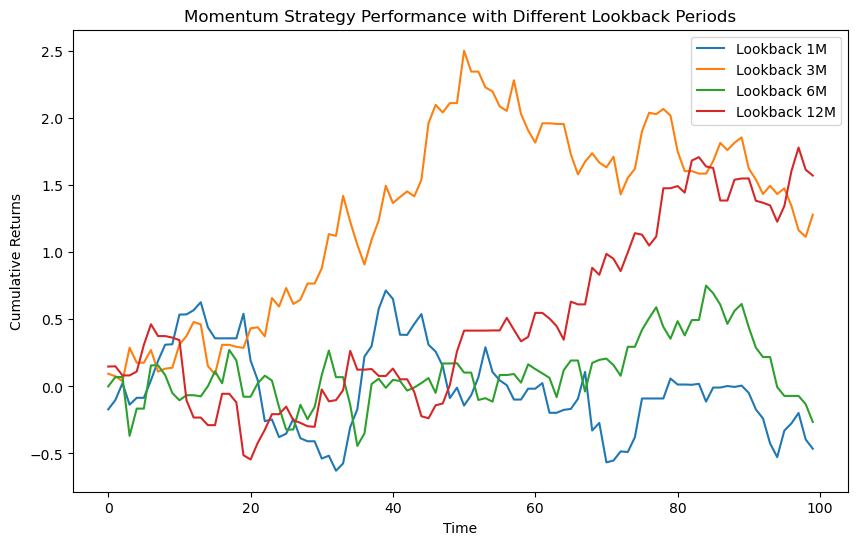
\includegraphics[width=0.8\textwidth]{Graphics/cum_returns_long_only.png}
    \caption[Cumulative Returns of Analyzed Lookback Periods]{This is the result of various lookback tested within our strategy. }
    \label{fig:my_label}
\end{figure}

\begin{table}[ht]
\centering
\caption{Example of a Simple Table}
\begin{tabular}{|c|c|c|} % alignment of each column data
\hline % horizontal line
\textbf{Lookback Period} & \textbf{Sharpe Ratio} & \textbf{Annual Return} \\ % header row
\hline
1 & X & Y \\
3 & X & Y \\
6 & X & Y \\
12 & X & Y \\

\hline
\end{tabular}
\end{table}

According to the Sharpe ratio, our data shows notable variations in the performance of momentum strategies for S\&P 100 companies over various look-back periods. With a Sharpe ratio of 6.40, the three-month lookback period performed better than the other periods, showing a larger risk-adjusted return than the one-, six-, and twelve-month periods, which had Sharpe rates of -0.26, 1.43, and 2.62, respectively. In contrast to the more erratic profiles of the one-month and six-month strategies, as well as the mediocre performance of the twelve-month strategy, the cumulative return chart demonstrates the superior performance of the three-month look-back strategy, which exhibits a more steady and noticeable upward trajectory of returns over time.

\section{Interpretation}
The three-month look-back period's excellent performance can be ascribed to its capacity to strike a balance between stability and reactivity. This time range is long enough to prevent the noise and overreaction that come with shorter time frames, yet short enough to respond swiftly to current market developments. The one-month period, on the other hand, is probably going to record too much market noise, creating a negative Sharpe ratio that denotes subpar risk-adjusted performance. Despite being more stable, the six- and twelve-month periods may not be as adept at taking advantage of short-term market changes, which is why their Sharpe ratios are lower than those of the three-month period. 

According to these findings, a three-month lookback period is the ideal length of time for momentum strategies in the S\&P 100 since it captures long-term trends well without being unduly impacted by transient market swings. For investors looking to maximize the effectiveness of their momentum-based investment strategies in equities markets, this result has significant ramifications, especially in settings with observable trend patterns and moderate volatility.


\printbibliography
\end{document}